\documentclass[main.tex]{subfiles}
\ifxetex\else\onlyinsubfile{\usepackage{CJKutf8}}\fi
\begin{document}
\ifxetex\else\begin{CJK*}{UTF8}{song}\fi

\chapter{内存管理(上)}
内存管理是操作系统的基本功能之一。在主流的操作系统中,一般都通过分页实现虚拟内存,给每个进程分配了一个巨大、连续、私有的虚拟内存,极大地简化了进程的内存管理。不仅如此,分页还允许进程之间共享内存,提高了物理内存的利用率。在 32位操作系统中, 4\-GiB的地址空间一般采用3:1布局,即 0~ 3\-GiB给用户代码,3~ 4\-GiB留给内核。

\par
本章讲解如何在 ARM上面实现基于分页的虚拟内存。

\section{物理内存布局}
在树莓派的物理内存布局中, SDRAM位于 0~ 0x2000\-0000 (512\-MiB),外围设备控制器的内存映射 I/O (Memory\--\-mapped I/O, MMIO)位于 0x2000\-0000~ 0x2100\-0000。截止到目前为止,物理内存的使用情况如图\ref{figure:4-1}所示。

\begin{figure}[htp]
\centering
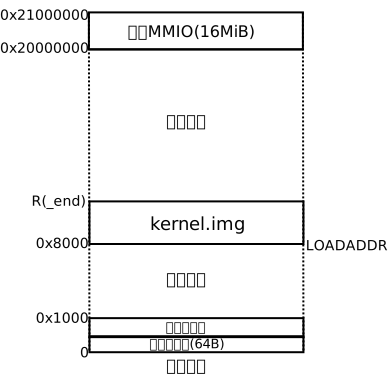
\includegraphics[scale=0.4]{figures/4-1}
\caption{物理内存使用情况}
\label{figure:4-1}
\end{figure}

\noindent
其中,异常向量表所占的 0~ 0x40共 64个字节是从 kernel.img的起始 64字节拷贝而来。符号 \_end定义在链接器脚本(代码\ref{code:2-5})中,它地址等于 kernel.img的结束地址。因为内核的链接地址从 0xc000\-8000开始,所以 \_end的地址等于 0xc000\-8000加上 kernel.img的大小。宏 R(x)=(x-0xc000\-0000)。

\section{页表结构}
 ARMv6支持多种页面大小,包括 4\-KiB、 64\-KiB、 1\-MiB和 16\-MiB,采用二级页表结构。一级页表分为 Section或 Page,二级页表分为 Large或 Small Page。如图\ref{figure:4-2}和\ref{figure:4-3}所示。

\begin{figure}[htp]
\centering
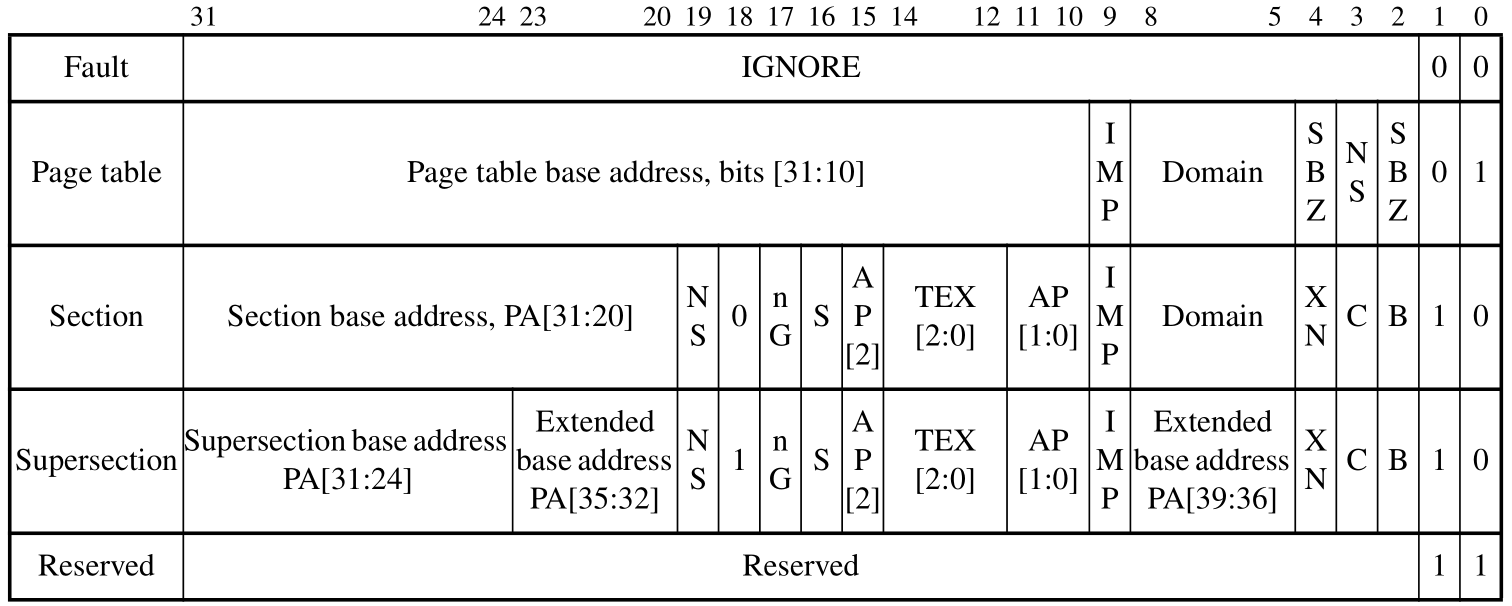
\includegraphics[scale=0.3]{figures/4-2}
\caption{ARMv6的一级页表项}
\label{figure:4-2}
\end{figure}

\begin{figure}[htp]
\centering
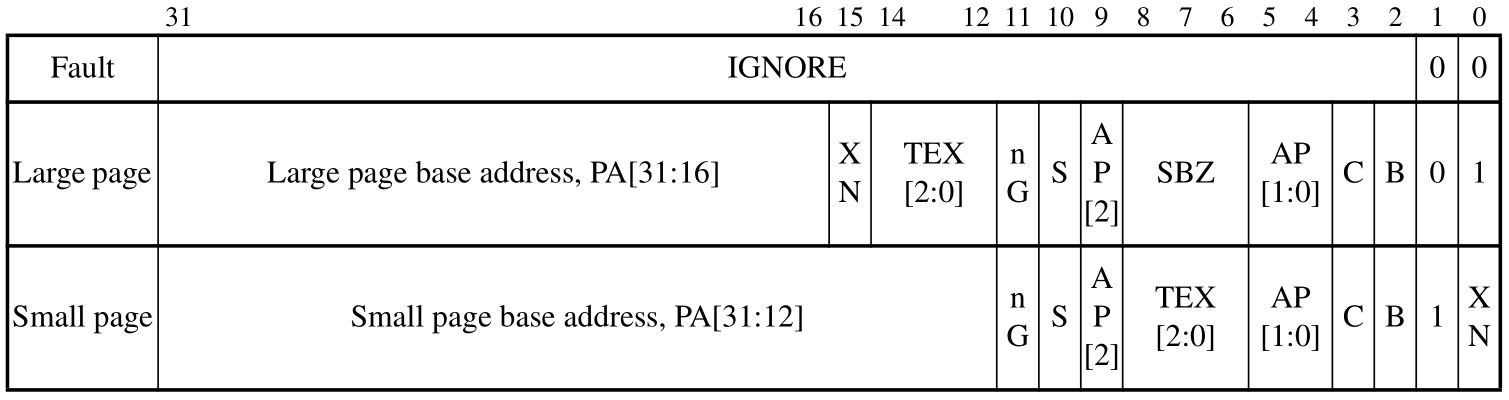
\includegraphics[scale=0.3]{figures/4-3}
\caption{ARMv6的二级页表项}
\label{figure:4-3}
\end{figure}

我们将采用 4\-KiB页面,对应于 Small Page结构,因此一级页表的大小是 16\-KiB,共 4096项;二级页表的大小是 1\-KiB,共 256项。从地址划分来看,这种结构意味着 32位的逻辑地址被分成了3段,第一段 12位,用于索引一级页表;第二段8位,用于索引二级页表;第三段12位,是页面内部的偏移量。图\ref{figure:4-4}给出了这种方案的地址转换过程。

\begin{figure}[htp]
\centering
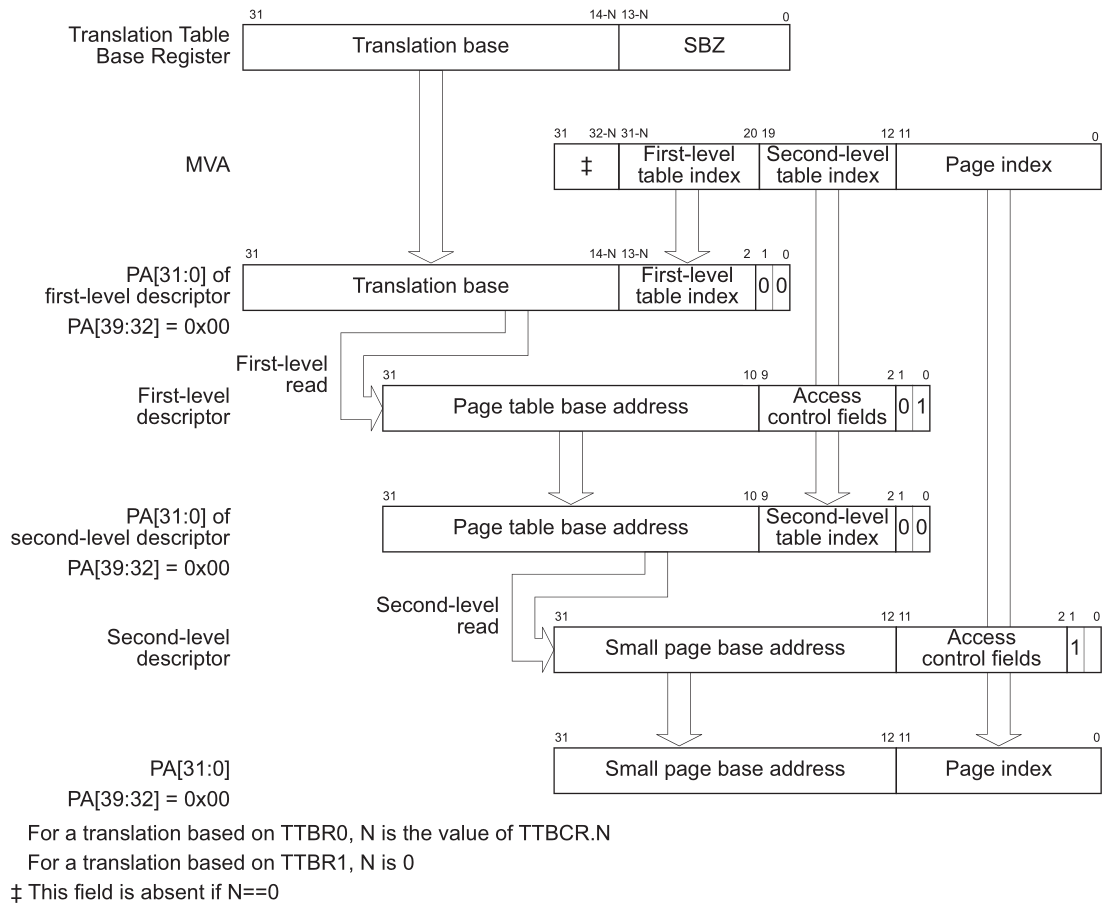
\includegraphics[scale=0.3]{figures/4-4}
\caption{地址转换过程(4KiB)}
\label{figure:4-4}
\end{figure}

\section{修改链接地址}
与大部分 32位的操作系统相同,我们也让内核运行在 3\-GiB (0xc000\-0000)以上的位置。也就是说, kernel.img被加载到物理地址 0x8000的位置,但我们要让它在 0xc000\-8000的逻辑地址上运行。

\par
在初始化页表之前,先要把内核 kernel.img链接到 0xc000\-8000。因为程序的逻辑地址是由链接器确定的。因此,要告诉链接器将内核链接到 0xc000\-8000,而不是原来的 0x8000。这只要修改链接器脚本 kernel.ld.in即可。在代码\ref{code:2-5}的基础上,只是添加了第2行、修改了第9行,如代码\ref{code:4-1}所示。

\begin{code}
\captionof{listing}{chapter04/kernel/kernel.ld.in}
\label{code:4-1}
\inputminted[firstline=1,lastline=12,linenos,numbersep=5pt,frame=lines,framesep=2mm]{c}{src/chapter04/kernel/kernel.ld.in}
\end{code}

修改链接地址后,相应地要修改 vector\_\-reset处的值。根据新的链接地址, \_entry的地址是 0xc000\-8000,而 reset的地址是 0xc000\-8040。 CPU复位时,这个地址显然是无效的,而真正有效的地址是 R(reset),即 0x8040。这正是代码\ref{code:4-2}中92行。由于相同的原因, 117~ 118行也进行了类似的修改。

\begin{code}
\captionof{listing}{chapter04/kernel/entry.S}
\label{code:4-2}
\inputminted[firstline=79,lastline=120,linenos,numbersep=5pt,frame=lines,framesep=2mm]{gas}{src/chapter04/kernel/entry.S}
\end{code}

重新编译之后,用命令“arm-\-none-\-eabi-\-objdump -D kernel.elf”查看反汇编的代码,可以发现所有的地址都被加上了 0xc000\-0000,如图\ref{figure:4-5}所示。

\begin{figure}[htp]
\centering
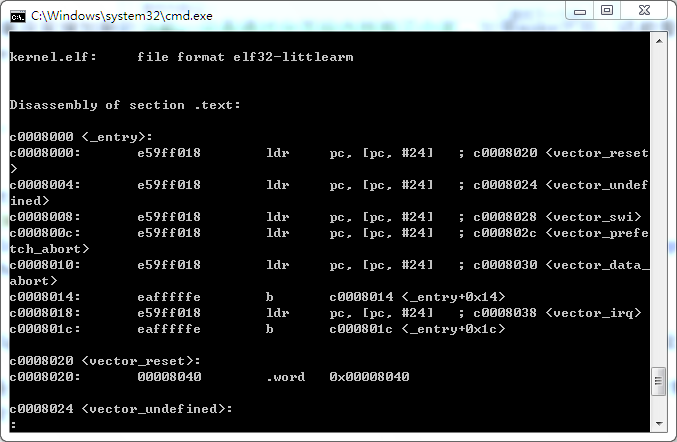
\includegraphics[scale=0.5]{figures/4-5}
\caption{内核链接到0xc0008000}
\label{figure:4-5}
\end{figure}

严格来说, kernel.img只有被加载地址 0xc000\-8000才能运行。然而,它被加载到 0x8000的位置,也可以运行。其原因在于编译器在产生代码的时候,会用相对地址。例如,图\ref{figure:4-5}中 \_entry处的几条指令,都是“ldr pc, [pc, \#24]”,这个指令的意思是:把 (PC+24)处4个字节的数据赋值给PC。因为树莓派的 CPU在复位时 PC=0x8000,这条指令会把 0x8020处(为什么不是 0x8018?因为在 ARM中 PC等于下一条指令的地址加8)的4字节数据赋值给PC,即 PC=0x8040。因此,这样的 kernel.img即使被加载到 0x8000也是可以运行的,因为通过相对地址避免了引用 0xc000\-8020这样的绝对地址。

\par
但是,不是所有的操作都可以用相对地址,例如访问全局变量一般会用到绝对地址。因为链接地址从 0xc000\-8000开始,这些位置显然没有任何内存,如果运行过程中引用了全局变量,就会导致程序出错。下面,我们通过初始化页表,让内核运行在被链接的逻辑地址之上。也就是说,我们要把内核从加载地址 0x8000重定位到逻辑地址 0xc000\-8000。注意,在初始化过程中,不能引用全局变量。

\section{页表初始化}
函数 init\_\-paging用于初始化页表,参数 phys\-free是空闲物理内存的起始地址。在我们的系统中,一级页表(也称为页目录)大小为 16\-KiB,保存着 4096张二级页表的物理地址。根据当前的内存使用状况(图\ref{figure:4-1}),把一级页表放物理内存 0x4000处。

\begin{code}
\captionof{listing}{chapter04/kernel/machdep.c}
\label{code:4-3}
\inputminted[firstline=145,lastline=157,linenos,numbersep=5pt,frame=lines,framesep=2mm]{c}{src/chapter04/kernel/machdep.c}
\end{code}

\noindent
 146~ 147行把一级页表的物理地址保存在变量 pgdir中,然后把内容全部清零。

\par
为了在逻辑地址空间中能够访问二级页表,要把它们映射到逻辑地址空间中。因为二级页表需要4MiB的逻辑地址 (4096张$\times$1\-KiB/张),我们决定把它们放在逻辑地址 [0xbfc0\-0000, 0xc000\-0000],而且它们自身也要消耗4张二级页表。代码\ref{code:4-4}分配了4张二级页表用来映射所有的二级页表。我们可以称这4张页表为二级页表的二级页表,这也是变量 ptpte的意义所在。因为二级页表全部位于逻辑地址 [0xbfc0\-0000, 0xc000\-0000],因此这4张特殊的二级页表应该分别被填到一级页表的 0xbfc(3068), 0xbfd(3069), 0xbfe(3070), 0xbff(3071)四项。需要特别解释一下第 162行,它保证了我们将来可以在逻辑地址空间中访问这4张特殊的二级页表。

\par
为了方便理解,这里列出各宏定义的值:PAGE\_\-SIZE=4\-KiB, L2\_\-TABLE\_\-SIZE=1\-KiB, PGDR\_\-SHIFT=20, (USER\_\-MAX\_\-ADDR\-\textgreater\textgreater\-PGDR\_\-SHIFT)=0xbfc(3068), L2\_\-ENTRY\_\-COUNT=1024。

\begin{code}
\captionof{listing}{chapter04/kernel/machdep.c}
\label{code:4-4}
\inputminted[firstline=159,lastline=170,linenos,numbersep=5pt,frame=lines,framesep=2mm]{c}{src/chapter04/kernel/machdep.c}
\end{code}

接下来,为内核地址空间(3\-GiB~ 4\-GiB)分配二级页表。尽管理论上需要 1024张二级页表,但是,实际上用不了那么多,因此目前只给它分配 80(即 NR\_\-KERN\_\-PAGETABLE)张。一张二级页表可以映射 1\-MiB的地址空间,这意味着可以映射 80\-MiB的逻辑地址空间,暂时已经足够用了。当然,我们要把二级页表的物理地址填充到一级页表中,而且所有的二级页表都要清零。此外,还要把新分配的二级页表以页面为单位(4张二级页表组成1个页面),填充到 ptpte中,保证将来用逻辑地址可以访问二级页表。注意,我们在填充一级页表的时候,把一级页表的第i项和 (i+0xc00)项填充成相同的值 (170行),这意味着逻辑地址x和 (0xc000\-0000+x)将被映射到相同的物理地址。二级页表项的标志位L2E\_\-V表示采用图\ref{figure:4-3}中的 Small page格式,L2E\_\-W表示可以写,L2E\_\-C表示可以被缓存。

\begin{code}
\captionof{listing}{chapter04/kernel/machdep.c}
\label{code:4-5}
\inputminted[firstline=172,lastline=185,linenos,numbersep=5pt,frame=lines,framesep=2mm]{c}{src/chapter04/kernel/machdep.c}
\end{code}

这样,我们就准备好了一、二级页表,如图\ref{figure:4-6}所示。

\begin{figure}[htp]
\centering
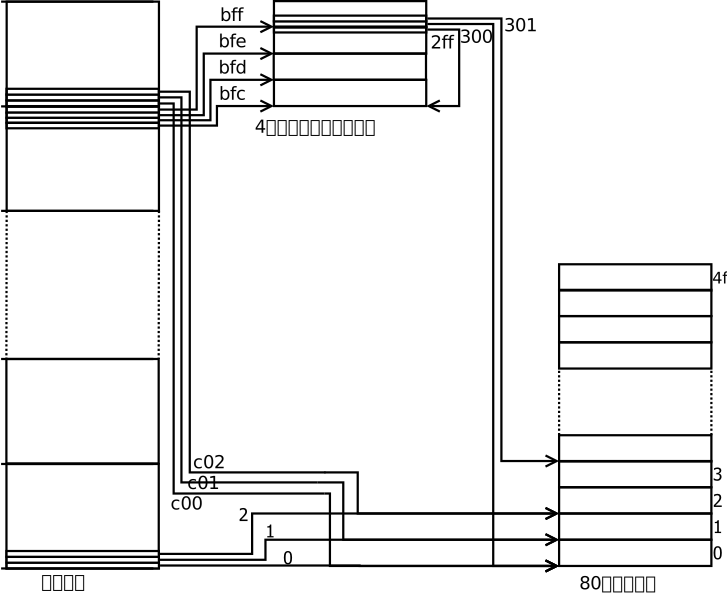
\includegraphics[scale=0.3]{figures/4-6}
\caption{一、二级页表组织}
\label{figure:4-6}
\end{figure}

\par
下面我们来填充二级页表。这部分比较简单,只要把物理内存从0开始、到 R(\_end)为止,以页面为单位,把物理地址按顺序填入对应的二级页表即可,如代码\ref{code:4-6}所示。

\begin{code}
\captionof{listing}{chapter04/kernel/machdep.c}
\label{code:4-6}
\inputminted[firstline=187,lastline=193,linenos,numbersep=5pt,frame=lines,framesep=2mm]{c}{src/chapter04/kernel/machdep.c}
\end{code}

根据前面一级页表的填充方式,意味着 0~ R(\_end)和 0xc000\-0000~ \_end这两段逻辑地址都映射到了物理地址 0~ R(\_end)。其中,前者是恒等映射,它保证了分页开启后的一段时间内,可以继续访问逻辑地址 0~ R(\_end)。当内核完全运行在 0xc000\-8000之后,就不需要恒等映射,届时将取消恒等映射。

\par
好了,现在已经填充了一、二级页表,接下来开启分页功能。首先,把一级页表的物理地址 pgdir填入 TTBR0寄存器,然后通过 TTBCR告诉 MMU;(1\textless\textless2)表示我们只用 Domain 1,而且把它的访问控制设置为“ Client”(=1),即所有内存访问都要进行权限检查; 在(1$\mid$(1\textless\textless23))中,1表示启动分页,(1\textless\textless23)的字面意思是禁止子页面访问权限检查,但因为只有 ARMv4和 ARMv5的页表结构支持子页面权限检查,所以(1\textless\textless23)表示只采用 ARMv6格式的页表结构。

\begin{code}
\captionof{listing}{chapter04/kernel/machdep.c}
\label{code:4-7}
\inputminted[firstline=195,lastline=217,linenos,numbersep=5pt,frame=lines,framesep=2mm]{c}{src/chapter04/kernel/machdep.c}
\end{code}

\noindent
一旦启动分页,所有的逻辑地址将被 MMU通过页表转换成物理地址。这也意味着, init\_\-paging返回后,内核可以在链接地址上运行,而且终于可以访问全局变量了。

\par
此时,物理、逻辑地址空间布局及其映射关系如图\ref{figure:4-7}所示。

\begin{figure}[htp]
\centering
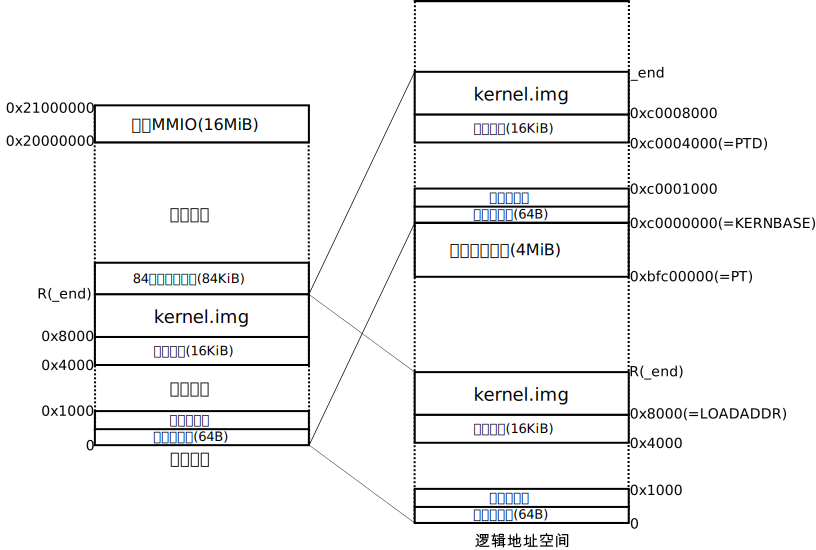
\includegraphics[scale=0.4]{figures/4-7}
\caption{物理、逻辑地址空间布局及其映射关系}
\label{figure:4-7}
\end{figure}

\section{物理内存管理}
启用分页后,从数值上来说,物理地址与逻辑地址之间已经没有什么关系了。为了记录物理内存和逻辑内存的使用状况,要分别对它们进行有效的管理。我们先从一个简单的物理内存管理器开始。

\par
考虑到物理内存在物理地址空间中不一定是连续的,我们定义一个全局的一维数组 g\_\-ram\_\-zone,用于记录系统可用的物理内存块。数组 g\_\-ram\_\-zone[2a]记录了一个内存块的起始地址, g\_\-ram\_\-zone[2a + 1]记录了它的结束地址。如果 g\_\-ram\_\-zone[2b]和 g\_\-ram\_\-zone[2b + 1]都是零,表示后面没有内存块了。我们给数组 g\_\-ram\_\-zone预留了 16(=RAM\_ZONE\_LEN)个元素,意味着最多可以保存7个物理内存块。由于树莓派只有一个物理内存块 [0,512\-MiB],只用了 g\_\-ram\_\-zone的4个元素,如代码\ref{code:4-8}所示。

\begin{code}
\captionof{listing}{chapter04/kernel/machdep.c}
\label{code:4-8}
\inputminted[firstline=219,lastline=228,linenos,numbersep=5pt,frame=lines,framesep=2mm]{c}{src/chapter04/kernel/machdep.c}
\end{code}

\noindent
参数 phys\-free是可用物理内存的起始地址,即 [0, phys\-free]部分的内存已经被使用,不能再用于分配。

\par
这个简单的数组只记录了系统可用的物理内存块,显然是不够的。在分页系统中,物理内存的最小分配单位是页面,所以要记录每一个页面的使用状况。因此,我们采用位图(bitmap)进行记录,即一个页面的状态用一位来表示,0表示空闲,1表示已分配。位图本身也需要占用物理内存,而且要在逻辑内存中能被访问。因此,我们根据物理内存区域的大小,为它创建位图,然后把位图映射到逻辑地址空间中来。

\par
对于每一个可用的物理内存区域,结构体 pm\-zone记录了它的起始地址、长度和位图指针。函数 init\_\-frame用于初始化物理内存管理器,它的参数 virt\-free是空闲逻辑内存的起始地址,用于映射位图。该函数调用了 page\_\-map,它定义于代码\ref{code:4-15}。

\begin{code}
\captionof{listing}{chapter04/kernel/frame.c}
\label{code:4-9}
\inputminted[firstline=23,lastline=54,linenos,numbersep=5pt,frame=lines,framesep=2mm]{c}{src/chapter04/kernel/frame.c}
\end{code}

下面来实现物理内存的分配函数 frame\_\-alloc。

\begin{code}
\captionof{listing}{chapter04/kernel/frame.c}
\label{code:4-10}
\inputminted[firstline=82,lastline=105,linenos,numbersep=5pt,frame=lines,framesep=2mm]{c}{src/chapter04/kernel/frame.c}
\end{code}

\par
物理内存的回收函数 frame\_\-free,功能正好相反,这里不再列出。

\section{逻辑内存管理}
与物理内存管理类似,我们用结构体 vmzone记录逻辑内存块的起始地址、长度和读写保护位。与物理内存相比,逻辑内存块的数量变化比较大,因此通过单向链表进行组织。

\begin{code}
\captionof{listing}{chapter04/kernel/page.c}
\label{code:4-11}
\inputminted[firstline=24,lastline=36,linenos,numbersep=5pt,frame=lines,framesep=2mm]{c}{src/chapter04/kernel/page.c}
\end{code}

逻辑地址空间由两部分组成,分别是用户、内核逻辑地址空间。用户逻辑地址空间是每个进程私有的,而内核地址空间是全局共享的。与此相对应,我们用 uvm\-zone和 kvm\-zone两个链表分别记录。注意,所有不在这两个链表记录范围内的逻辑内存,都是不可访问的。

\par
函数 init\_\-vmspace初始化两个链表,参数 virt\-free是此时内核所用逻辑内存块的结束地址。因为此时内核已经用了一块逻辑内存 [0xbfc0\-0000, virt\-free](即从二级页表开始到 virt\-free结束),我们把这块内存的信息保存到静态变量 km0,并作为 kvm\-zone链表的第一个节点。而用户的逻辑地址空间是空的,所以把 uvm\-zone初始化为 NULL。

\begin{code}
\captionof{listing}{chapter04/kernel/page.c}
\label{code:4-12}
\inputminted[firstline=38,lastline=47,linenos,numbersep=5pt,frame=lines,framesep=2mm]{c}{src/chapter04/kernel/page.c}
\end{code}

现在我们来实现逻辑内存块的分配函数,即 page\_\-alloc。它的参数 npages表示需要的页面个数, prot表示读写保护位, user指示从用户空间、还是从内核空间分配。注意,这个函数调用了 kmalloc,它从内核堆中分配内存。内核堆的管理,将在本章稍后讲解。为什么代码\ref{code:4-12}中的 km0不能用 kmalloc分配呢?因为彼时还没有初始化内核堆。

\begin{code}
\captionof{listing}{chapter04/kernel/page.c}
\label{code:4-13}
\inputminted[firstline=112,lastline=174,linenos,numbersep=5pt,frame=lines,framesep=2mm]{c}{src/chapter04/kernel/page.c}
\end{code}

\noindent
函数 page\_\-alloc的返回值是新分配的内存块在逻辑地址空间中的起始地址。此外,我们经常需要在指定的地址分配逻辑内存块,这正是函数 page\_\-alloc\_\-in\_\-addr的功能。

\begin{code}
\captionof{listing}{chapter04/kernel/page.c}
\label{code:4-14}
\inputminted[firstline=49,lastline=110,linenos,numbersep=5pt,frame=lines,framesep=2mm]{c}{src/chapter04/kernel/page.c}
\end{code}

我们还定义了两个函数: page\_\-map和 page\_\-unmap。函数 page\_\-map把指定的逻辑地址映射到指定的物理地址,而 page\_\-unmap取消这种映射。

\begin{code}
\captionof{listing}{chapter04/kernel/page.c}
\label{code:4-15}
\inputminted[firstline=239,lastline=252,linenos,numbersep=5pt,frame=lines,framesep=2mm]{c}{src/chapter04/kernel/page.c}
\end{code}

\noindent
因为修改了页表项中的地址映射,我们用函数 invlpg(va)清空TLB缓存中逻辑地址 va的缓存项。

\par
这里着重说明一下 vtopte(va)。它其实是个宏定义,计算给定逻辑地址 va所对应的二级页表项的指针。把代码\ref{code:4-16}和\ref{code:4-17}放在一起看,才能更好地理解 vtopte。其中, PGDR\_\-SHIFT=20, PAGE\_\-SHIFT=12,全局变量 PTD指向了一级页表的起始地址,即 0xc000\-4000;而PT指向了二级页表的起始地址,即 0xbfc0\-0000,如图\ref{figure:4-7}所示。

\begin{code}
\captionof{listing}{chapter04/kernel/kernel.h}
\label{code:4-16}
\inputminted[firstline=38,lastline=48,linenos,numbersep=5pt,frame=lines,framesep=2mm]{c}{src/chapter04/kernel/kernel.h}
\end{code}

\begin{code}
\captionof{listing}{chapter04/kernel/kernel.c}
\label{code:4-17}
\inputminted[firstline=13,lastline=14,linenos,numbersep=5pt,frame=lines,framesep=2mm]{c}{src/chapter04/kernel/kernel.c}
\end{code}

\section{缺页异常处理}\label{section:page-fault}
启动分页后,逻辑地址与物理地址是两个独立的地址空间,它们之间通过页表进行映射。程序中引用的地址都是逻辑地址。如果访问的逻辑地址已经被映射到了物理内存,程序能正常执行。否则, CPU会触发一个缺页异常。缺页异常对于实现虚拟内存是必须的,但是本章只实现了逻辑内存到物理内存的映射,而不实现涉及输入输出的页面置换、交换等功能。

\par
在 ARM中,有两个缺页异常,分别是 pre\-fetch和 data abort。其中, pre\-fetch abort是从内存中预取指令时引起的,而data abort是访问内存数据引起的。

\par
首先,要修改 entry.S中的异常向量表,加上 pre\-fetch和 data abort入口,如代码\ref{code:4-18}所示。

\begin{code}
\captionof{listing}{chapter04/kernel/entry.S}
\label{code:4-18}
\inputminted[firstline=91,lastline=106,linenos,numbersep=5pt,frame=lines,framesep=2mm]{gas}{src/chapter04/kernel/entry.S}
\end{code}

在处理这两个异常时,仍然使用 PUSH\-CONTEXT和 PULL\-CONTEXT两个宏定义,因为这部分的处理方法与中断是完全相同的。需要特别注意的是, IRQ和 pre\-fetch abort时lr\_\-irq和lr\_\-abt等于 (PC+4),而 data abort时 lr\_\-abt等于 (PC+8),因此在 PUSH\-CONTEXT之前,先要把 lr减掉4才能进行后续的统一处理。

\par
接着,把缺页异常发生时的 CPU现场 (struct context)、以及触发该异常的逻辑地址 (Fault Address, FA)和状态码 (Fault Status, FS)作为参数传递给统一的C语言处理函数 abort\_\-handler。

\begin{code}
\captionof{listing}{chapter04/kernel/entry.S}
\label{code:4-19}
\inputminted[firstline=157,lastline=178,linenos,numbersep=5pt,frame=lines,framesep=2mm]{gas}{src/chapter04/kernel/entry.S}
\end{code}

现在我们来看看 abort\_\-handler。它只是调用 do\_\-page\_\-fault处理缺页异常,如果 do\_\-page\_\-fault返回0表示成功处理了该异常,可以继续运行;否则调用函数 panic打印信息,供调试使用。

\begin{code}
\captionof{listing}{chapter04/kernel/machdep.c}
\label{code:4-20}
\inputminted[firstline=329,lastline=335,linenos,numbersep=5pt,frame=lines,framesep=2mm]{c}{src/chapter04/kernel/machdep.c}
\end{code}

因此,所有缺页异常的逻辑都是在 do\_\-page\_\-fault中实现的。它首先根据状态码判断触发异常的原因。原因大体上可以分成三类:对齐 (alignment),转换 (translation),权限 (permission)。目前,我们只处理了 translation fault,即逻辑内存未映射到物理内存导致 MMU不能完成地址转换,其他未处理的情况都返回失败。然后,用 page\_\-prot判定触发异常的逻辑地址是否位于有效的逻辑内存块内,即该地址是否位于 vm\-zone链表所记录的逻辑内存范围内。如果不是,表示访问了非法的逻辑内存,返回失败;否则,调用 frame\_\-alloc分配一个物理内存页面。如果没有空闲的物理内存,也返回失败。接着,通过修改页表把触发异常的逻辑地址所在的页面映射到新分配的物理内存上,结束了一次异常处理的流程。

\par
显然,对于二级页表本身引起的缺页异常,要把新分配的二级页表的物理地址填充到一级页表中。特别注意,1个页面可以容纳4张二级页表。

\begin{code}
\captionof{listing}{chapter04/kernel/machdep.c}
\label{code:4-21}
\inputminted[firstline=256,lastline=327,linenos,numbersep=5pt,frame=lines,framesep=2mm]{c}{src/chapter04/kernel/machdep.c}
\end{code}

\section{内存管理初始化}
前面几节,我们完成了页表初始化、物理内存和逻辑内存管理、缺页异常的处理。下面把这些功能组合起来,完成整个内存管理系统的初始化工作。

\subsection{修改栈地址}
在本章之前,各个模式的栈位于 0x1000之下(参考代码\ref{code:3-4})。从本章开始,因为内核被链接到了 3\-GiB之上,也要相应地修改栈的地址,将来才能以链接地址运行。修改方法是在原来的地址上,全部加上 KERN\-BASE (=3\-GiB),如代码\ref{code:4-22}所示。注意,我们没有修改 supervisor模式的栈,因为在尚未开启分页之前, CPU运行在该模式。而其他模式的栈,当启用分页之后才会访问,可以先行修改。

\begin{code}
\captionof{listing}{chapter04/kernel/entry.S}
\label{code:4-22}
\inputminted[firstline=127,lastline=144,linenos,numbersep=5pt,frame=lines,framesep=2mm]{gas}{src/chapter04/kernel/entry.S}
\end{code}

\subsection{启用分页}
回到内核的C语言入口函数 cstart。因为要尽快启用分页,所以进入 cstart后的第一件事就是调用前面的 init\_\-paging初始化页表并启用分页。全局符号 end定义在链接器脚本中(参考代码\ref{code:2-5}),它的地址,即局部变量 \_end=KERN\-BASE+kernel.img的大小,宏 R(x)=x-KERN\-BASE。局部变量 phys\-free保存着内核被加载到物理内存的结束地址,亦即空闲物理内存的起始地址,而且通过 PAGE\_\-ROUNDUP把它向上取整到页面大小(即 4\-KiB)的倍数。

\begin{code}
\captionof{listing}{chapter04/kernel/machdep.c}
\label{code:4-23}
\inputminted[firstline=347,lastline=355,linenos,numbersep=5pt,frame=lines,framesep=2mm]{c}{src/chapter04/kernel/machdep.c}
\end{code}

因为 init\_\-paging在初始化页表的时候要消耗掉一部分物理内存,因此它返回了新的空闲物理内存的起始地址。

\par
函数 init\_\-paging返回后,分页已经被开启。此时系统还能正常运行,原因就在于页表中的恒等映射,它保证了逻辑地址等于物理地址。另一方面,逻辑地址 (x+KERN\-BASE)也被映射到了物理地址x。

\par
下面,我们切换到逻辑地址运行。切换工作由函数 trampoline完成。单词 trampoline的字面意思是蹦床,这正是该函数完成的功能,即从加载地址x蹦到逻辑地址 (x+KERN\-BASE)上去。

\begin{code}
\captionof{listing}{chapter04/kernel/machdep.c}
\label{code:4-24}
\inputminted[firstline=357,lastline=360,linenos,numbersep=5pt,frame=lines,framesep=2mm]{c}{src/chapter04/kernel/machdep.c}
\end{code}

这个函数的修饰符“\_\_\-attribute\_\_\-((naked))”告诉编译器不要为它生成出入口代码,函数内部只是把 sp和 lr寄存器加上 KERN\-BASE,然后用“bx lr”指令返回。显然,函数返回之后 sp和 pc都被加上了 KERN\-BASE,这就意味着之后的代码,已经以逻辑地址运行了。

\begin{code}
\captionof{listing}{chapter04/kernel/machdep.c}
\label{code:4-25}
\inputminted[firstline=337,lastline=345,linenos,numbersep=5pt,frame=lines,framesep=2mm]{c}{src/chapter04/kernel/machdep.c}
\end{code}

\subsection{物理及逻辑内存初始化}
接下来,先后调用 init\_\-ram和 init\_\-frame初始化物理内存管理器。根据图\ref{figure:4-7}, \_end是空闲逻辑内存的起始地址,把它向上取整到页面大小的倍数后,传给 init\_\-frame用于映射空闲物理内存的位图。 init\_\-frame返回新的空闲逻辑内存的起始地址。然后,调用 init\_\-vmspace初始化内核和用户逻辑内存管理器。

\par
在内核运行过程中,也需要动态地分配和释放内存,有必要开辟一块逻辑内存作为内核堆。因此, init\_\-vmspace在内核的逻辑内存中预留了 4\-MiB给内核堆使用。注意,这里只给堆分配了地址空间,并未分配物理内存。将来访问堆时,通过\ref{section:page-fault}节实现的缺页异常处理,自动完成物理内存的分配以及逻辑内存到物理内存的映射。

\par
初始化内核堆是通过调用 init\_\-kmalloc完成的。我们采用了著名的堆分配器\htmladdnormallink{TLSF}{http://www.gii.upv.es/tlsf/}(Two-Level Segregated Fit allocator)管理内核堆。 TLSF提供了malloc/\-realloc/\-memalign/\-free等标准的接口,这里只是根据需要做了简单的封装。

\begin{code}
\captionof{listing}{chapter04/kernel/machdep.c}
\label{code:4-26}
\inputminted[firstline=362,lastline=377,linenos,numbersep=5pt,frame=lines,framesep=2mm]{c}{src/chapter04/kernel/machdep.c}
\end{code}

\subsection{映射外设地址}
在第二、三章中,我们通过访问 MMIO内存块 [0x2000\-0000, 0x2100\-0000]控制外设。启用分页之后,这个逻辑内存块并未被映射到物理内存,不能再直接用它们控制外设了。为此,要把 MMIO内存映射到逻辑地址空间中来,然后才能用逻辑地址去访问外设。把 MMIO内存映射到哪个逻辑内存块呢?前面讲过,我们给内核分配了 80张二级页表,能映射 80\-MiB地址空间,即 0xc000\-0000~ 0xc500\-0000。为了充分利用这 80张页表,我们把 MMIO内存映射到逻辑地址 [0xc400\-0000,  0xc500\-0000]。选择了映射地址之后,通过 page\_\-alloc\_\-in\_\-addr把这一块逻辑内存登记到地址空间 vm\-zone中,然后调用函数 page\_\-map完成映射关系。需要特别注意的是,在调用 page\_\-map时,页表项标志位 flags不能带L2E\_\-C,这是因为 MMIO内存不能被缓存。

\begin{code}
\captionof{listing}{chapter04/kernel/machdep.c}
\label{code:4-27}
\inputminted[firstline=379,lastline=384,linenos,numbersep=5pt,frame=lines,framesep=2mm]{c}{src/chapter04/kernel/machdep.c}
\end{code}

除此之外,还得把源代码中的“MMIO\_\-BASE\_\-PA+XXX\_\-REG”的地方全部改为“MMIO\_\-BASE\_\-VA+XXX\_\-REG”,然后才能正常访问外设。

\subsection{开启 HiVecs功能}
在 ARM早期的版本中,异常向量的基地址只能是0,即复位时 PC=0、 IRQ时 PC=0x18等等,如图\ref{figure:4-8}所示。所以,内核必须保留逻辑地址空间的第一个页面 [0, 0x1000]用于放置异常向量。在 ARM\-720T之后,支持所谓的 Hi\-Vecs,即异常向量的基地址可以是 0xffff\-0000。开启 Hi\-Vecs后,复位时 PC=0xffff\-0000、 IRQ时 PC=0xffff\-0018等等,见图\ref{figure:4-8}。

\begin{figure}[htp]
\centering
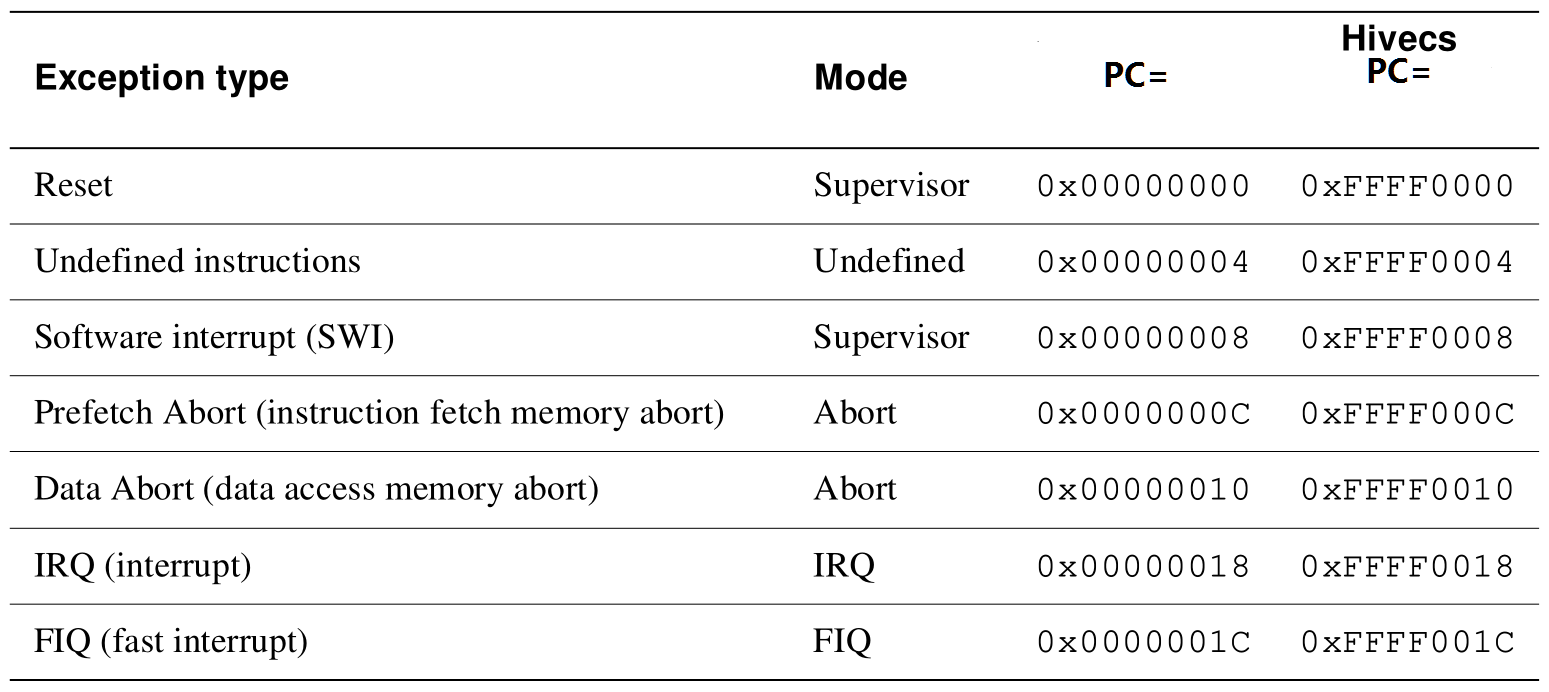
\includegraphics[scale=0.3]{figures/4-8}
\caption{触发异常时PC的值}
\label{figure:4-8}
\end{figure}

因此,我们先把 [0xffff\-0000, 0xffff\-1000]这一个页面用 page\_\-alloc\_\-in\_\-addr预留下来,然后用 page\_\-map把它映射到物理地址 0x8000(因为异常向量表位于 kernel.img的开始位置,而 kernel.img被加载到物理地址 0x8000)。这样就把异常向量挪到了逻辑地址 0xffff\-0000上,然后通过修改系统控制寄存器 SCTLR开启 Hi\-Vecs模式。

\begin{code}
\captionof{listing}{chapter04/kernel/machdep.c}
\label{code:4-28}
\inputminted[firstline=386,lastline=404,linenos,numbersep=5pt,frame=lines,framesep=2mm]{c}{src/chapter04/kernel/machdep.c}
\end{code}

\subsection{取消恒等映射}
经过前面的初始化步骤,内核已经运行于设定的链接地址,而且中断和缺页异常发生时,会直接跳转到 Hi\-Vecs,不再需要恒等映射。取消恒等映射很简单,只要把一级页表的前 80 (= NR\_\-KERN\_\-PAGE\-TABLE)项全部清零即可,代码\ref{code:4-29}中的全局变量 PTD是指向一级页表的指针。然后,清空整个 TLB缓存,以使修改立即生效。

\begin{code}
\captionof{listing}{chapter04/kernel/machdep.c}
\label{code:4-29}
\inputminted[firstline=406,lastline=418,linenos,numbersep=5pt,frame=lines,framesep=2mm]{c}{src/chapter04/kernel/machdep.c}
\end{code}

至此,物理内存和逻辑内存的布局如图\ref{figure:4-9}所示。

\begin{figure}[htp]
\centering
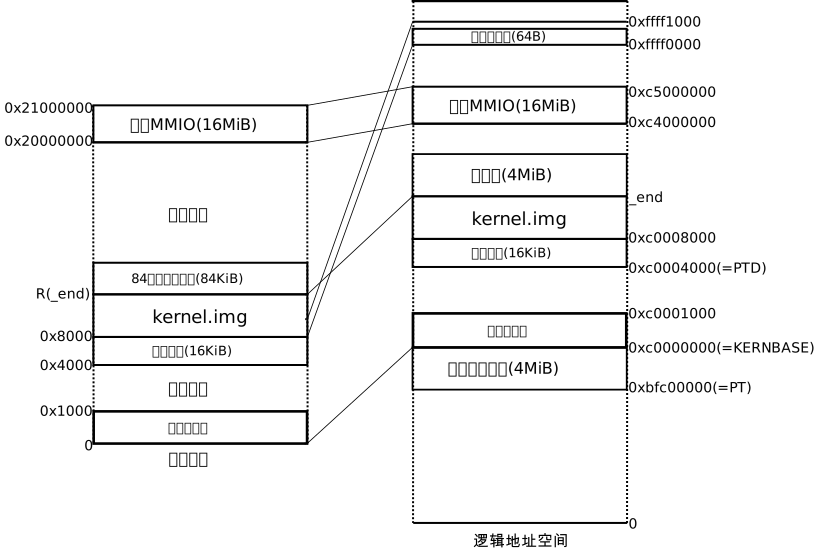
\includegraphics[scale=0.4]{figures/4-9}
\caption{物理内存和逻辑内存的布局}
\label{figure:4-9}
\end{figure}

\section{测试}
从表面上看,本章没有增加新的功能,只是通过分页给内核搬了个家。如果 make之后,还能看到图\ref{figure:3-6}的输出,表明搬家成功了。

\par
为了进一步验证,我们用代码\ref{code:4-30}进行了简单的测试。

\begin{code}
\captionof{listing}{chapter04/kernel/machdep.c}
\label{code:4-30}
\inputminted[firstline=448,lastline=458,linenos,numbersep=5pt,frame=lines,framesep=2mm]{c}{src/chapter04/kernel/machdep.c}
\end{code}

结果如图\ref{figure:4-10}所示。其中,点“.”是定时器中断处理函数的输出。因为用户地址空间 [0, 0xbfc0\-0000)是空的,所以 446行访问0地址时会触发无法处理的缺页异常。注意,中断或异常发生时, CPU会自动屏蔽中断 (CPSR.I=1),所以后面看不到定时器中断的输出。

\begin{figure}[htp]
\centering
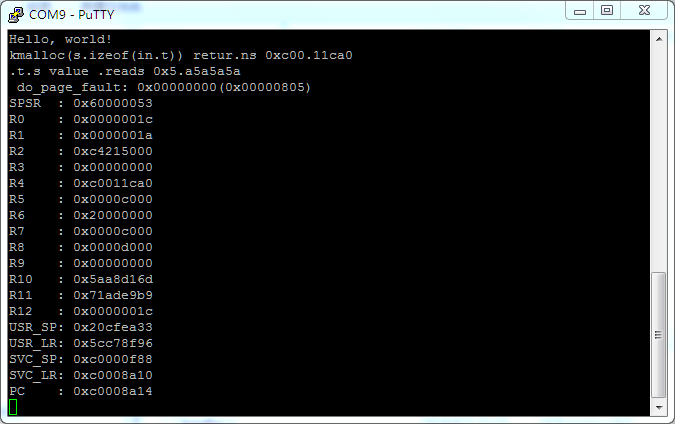
\includegraphics[scale=0.5]{figures/4-10}
\caption{测试结果输出}
\label{figure:4-10}
\end{figure}

从打印的信息可以看到,引起缺页异常的地址是 0x0000\-0000,状态码 0x0000\-0805表示 translation section fault。这是因为0地址的页表项所在的二级页表没有映射到物理内存。

\par
根据 PC寄存器的值,我们知道访问0地址发生在 0xc000\-8a14位置。图\ref{figure:4-11}是命令“arm-\-none-\-eabi-\-objdump -D kernel.elf”的输出,从中可以看出 0xc000\-8a14正是对应源代码446行中“*p = 0”的语句。

\begin{figure}[htp]
\centering
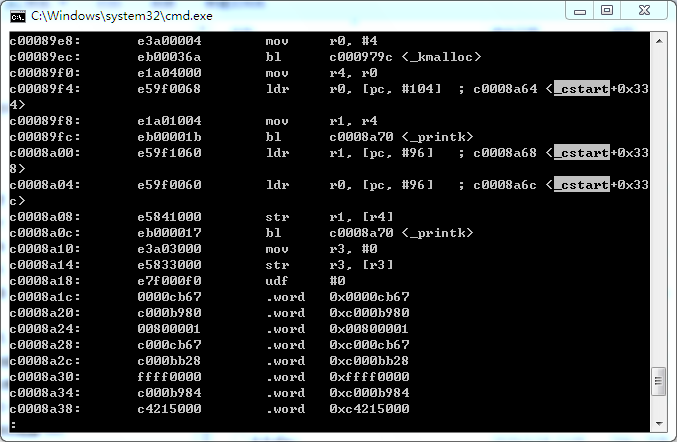
\includegraphics[scale=0.5]{figures/4-11}
\caption{通过PC寄存器找到异常发生时正在执行的指令}
\label{figure:4-11}
\end{figure}

\section{小结}
本章通过分页实现了一个基本的内存管理框架。尽管没有增加系统的功能,但是为后续开发准备了立脚点。

\clearpage
\ifxetex\else\end{CJK*}\fi
\end{document} 